\documentclass[10pt,letterpaper]{article}
\usepackage[T1]{fontenc}
\renewcommand{\rmdefault}{ptm}
\renewcommand{\ttdefault}{pcr}
\usepackage[letterpaper,left=1.06in,right=1.06in,top=.89in,bottom=.89in]{geometry}
\usepackage{amsmath,amssymb,graphicx,booktabs}
\usepackage[hidelinks]{hyperref}
\hypersetup{pdftitle={One-exposure recovery bounds after the 2024 Juice lunar flyby},pdfauthor={Adam Cohen}}
\newcommand{\degc}{^{\circ}}
\newcommand{\as}{^{\prime\prime}}
\newcommand{\norm}[1]{\left\lVert #1\right\rVert}
\newcommand{\dotp}{\mathbin{\cdot}}
\newcommand{\doi}[1]{\href{https://doi.org/#1}{doi:\,#1}}
\DeclareMathSizes{10}{10}{7}{7}
\setlength{\emergencystretch}{2em}
\setlength{\parindent}{1.1em}
\setlength{\parskip}{2pt}
\linespread{1.06}
\raggedbottom
\begin{document}
\begin{center}
{\LARGE\bfseries One-exposure recovery bounds after the\\[3pt] 2024 Juice lunar flyby\par}
\vspace{9pt}
{\large Adam Cohen}\\[2pt]
Orbital Engineering Lab\\[4pt]
{\small Manuscript draft \quad 19 November 2026}
\end{center}

\begin{abstract}\normalsize
A least-squares orbit fitted to 25 optical observations of ESA's Juice spacecraft predicted its direction after the 2024 lunar flyby to within $0.0503\degc$ of the JPL reconstruction. Yet centering an ideal, freely rotatable $4.4\degc$ square on that prediction misses an admissible direction at every roll. At a hard $2.00\as$ residual cap per exposure, the direction lies at least $3.18018\degc$ from the prediction, beyond the $3.10974\degc$ corner radius. A $0.20557\degc$ pointing change covers the modeled family in a numerical enclosure of 638 incoming regions. The minimum square side is between $4.314\degc$ and $4.400\degc$. Under point-mass lunar gravity and a spherical surface, three compatible orbits exclude every pointing by $2.148\as$, although each pair fits. A terrain and lunar-gravity replay rejects one of those orbits. A nearby replacement clears the sampled terrain and recovers the three-direction obstruction numerically. These caps bracket a transition for the selected arc and nominal model. A single exposure from the preceding night rejects all four nominal orbits used to demonstrate the two failures.

\end{abstract}

\section{Introduction}
An optical orbit fit can predict where to point a telescope. During a close encounter, small changes in incoming range or velocity can change the gravitational deflection enough to move the outgoing direction across the detector. An accurate best-fit prediction then leaves a separate question unanswered. Could a single exposure have covered every direction allowed by the original data?

Milani formulated asteroid recovery as the nonlinear image on the sky of a region of compatible orbits \cite{milani}. Espitia et al.\ tested triangulated admissible regions against a rectangular field in asteroid recovery observations \cite{espitia}. Pirovano et al.\ represented families of optically compatible orbits as continuous sets \cite{piro}. Wittig et al.\ propagated large uncertainty sets through nonlinear encounters by polynomial expansion and domain splitting \cite{wittig}. For Juice itself, Benedikter et al.\ fitted six angles from August 7 and 9 with deterministic initial orbit determination and differential correction \cite{tracer}. The flight navigation team reconstructed the August 19 lunar encounter using mission tracking \cite{dietz}.

We use a later, publicly archived optical arc to bound a detector decision on both sides. For sufficiency, one specified camera must contain the entire surviving family. For exclusion, a finite number of feasible trajectories can suffice, provided every camera placement fails. The square introduces a useful distinction. Its diagonal can accommodate directions farther apart than its side, but different pairs can require incompatible orientations. Figure~\ref{fig:decision} shows the consequence for the observer. The best-fit pointing misses one compatible orbit at every roll, while a shift of about twelve arcminutes places the whole nominal family inside the field. We also test whether the trajectories responsible for the all-pointings exclusion survive a measured lunar shape and a rotating gravity field.

\begin{figure}[htbp]
\centering
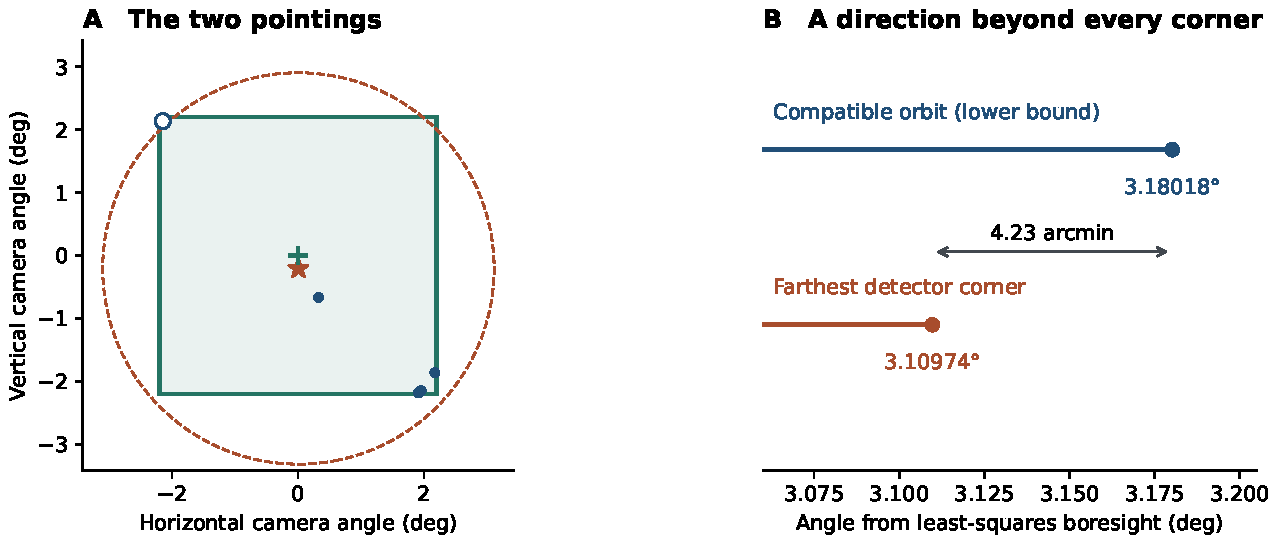
\includegraphics[width=.94\linewidth]{detector-decision.pdf}
\caption{Why the least-squares pointing fails at $2.00\as$. In panel A the star is the best-fit prediction and the dashed circle passes through the farthest corners available at that boresight for any roll. The open blue marker identifies a verified orbit outside this circle. The shaded square, centered on the cross, shows the sufficient placement. Blue dots are individual verified directions. Panel B subtracts the orbit's forecast error radius before comparing its distance with the camera corner.}
\label{fig:decision}
\end{figure}

\section{Observations, dynamics and detector}

The training set comprises 25 distinct, unflagged optical directions in the Project Pluto archive for 2023-053A, entries 75--99 \cite{astrometry}. They span 48.10 hours from August 15 at 07:27:53.856 UTC to August 17 at 07:33:53.280 UTC. Observatory codes 718, C23, C40 and Y05 contributed 14, five, three and three directions, respectively. Six incoming range and range-rate seeds were used to initialize the optical fit. The prediction epoch was August 20 at 06:00 UTC at observatory 703, about 8 h 45 min after lunar closest approach and before the Earth encounter. The cutoff, site and epoch were fixed before the initial forecast was scored. The ephemeris correction and the detector-bound searches described below were retrospective.

Let $x$ be the six-component geocentric inertial state at first reception. Write $R_E(t)$ for Earth's barycentric position, $r_x(t)$ for the propagated geocentric position and $r_i(t_i)$ for the geocentric observing site at reception. The astrometric ray $y_i$, light time and unit direction satisfy
\begin{equation}
 y_i=R_E(\tau_i)+r_x(\tau_i)-R_E(t_i)-r_i(t_i),\qquad
 c_0(t_i-\tau_i)=\norm{y_i},\qquad u_i(x)=y_i/\norm{y_i},
 \label{eq:light}
\end{equation}
where $c_0$ is the speed of light. The station rotation uses Earth orientation at the recorded epoch. The same observation map defines $u_*(x)$ for the prediction site and time. Sky residuals are great-circle angles to the observed unit directions $v_i$. Thus $\epsilon$ bounds the two-dimensional angular discrepancy at \emph{each} exposure, including the least favorable one.

For the least-squares fit, let $e_i,n_i$ be the local east and north unit vectors at $v_i$. The optimizer minimizes the sum of squares of the 50 tangent coordinates $(u_i\dotp e_i,u_i\dotp n_i)/(u_i\dotp v_i)$ with equal weight. During this fit it approximates the emission position using constant barycentric velocity over the light time. A local refit that propagated the spacecraft to iterated emission times and interpolated Earth's displacement shifted the post-flyby boresight by $0.0067$--$0.0071\as$ across three finite-difference step sizes. The fixed-boresight miss below is $4.226$ arcminutes.

The Orbital Engineering Lab (OEL) Numerical Propagator integrates passive motion under Earth central gravity and $J_2$, with lunar and solar point-mass third-body gravity. The compact DE440s ephemeris supplies body positions. An initial resource used a lunar vector relative to the Earth--Moon barycenter where the dynamics required a geocentric vector. Rebuilding the resource reduced the lunar position discrepancy against a geocentric JPL vector at the encounter from 4,395 km to 2.31 m. All calculations use the corrected resource. The whole-set enclosure uses the nominal force law. Section~\ref{sec:lunar} changes the lunar field and surface for individual trajectories. An OEL coast initialized at JPL's reconstructed first-epoch state differed from the reconstructed final direction by $12.75\as$, giving a separate check on combined model and reference disagreement \cite{horizons}.

Define $\mathcal A_\epsilon$ to be the states satisfying all 25 residual inequalities $\angle(u_i(x),v_i)\leq\epsilon$ and the following physical priors. Over the observed arc and emission lookback, geocentric distance is at least 200,000 km and lunar-centered distance at least 100,000 km. Geocentric speed is at most 6 km/s through the prediction epoch. Trajectories must remain exterior to Earth and to a lunar sphere of radius 1,737.4 km. Clock offsets and angular station biases are fixed at their nominal values. The set of possible sky directions is $\mathcal U_\epsilon=\{u_*(x):x\in\mathcal A_\epsilon\}$.

Catalina's 703 Schmidt camera has 10,560 pixels on a side at a nominal $1.5\as$ per pixel \cite{camera}. We model it as a filled tangent-plane square with angular side $s=4.4\degc$ across opposite edge midpoints. For a unit boresight $b$ and orthonormal rolled tangent axes $e_1,e_2$, a forward direction $u$ is inside exactly when
\begin{equation}
 (\sigma e_k-b\tan(s/2))\dotp u\leq 0,\qquad k=1,2,\quad \sigma\in\{-1,1\}.
 \label{eq:faces}
\end{equation}
The minimum side $s_*(\epsilon)$ is the infimum of $s$ for which some $b,e_1,e_2$ satisfy Eq.~\eqref{eq:faces} for every $u\in\mathcal U_\epsilon$. The corresponding minimum circular diameter is $d_*(\epsilon)$. A containing square immediately gives a containing circle of diameter $2\arctan(\sqrt{2}\tan(s/2))$.

\section{Enclosing all surviving directions}

\subsection{Incoming optical constraints}
At each exposure the unknowns are the three position components, three velocity components and a positive light-path range. The 25 receptions give 175 variables. The speed limit and the change in sight lines bound range. Integrating the equations of motion between receptions couples adjoining states. To constrain Eq.~\eqref{eq:light}, expansion about reception retains the range times the sum of Earth and spacecraft velocity divided by $c_0$. Linear inequalities bound each range--velocity product on its coordinate intervals. Tangent inequalities in several azimuths enclose each circular measurement cap from outside. A state satisfying the optical model remains feasible after these relaxations.

The long gaps between observing nights control how much spurious range and range-rate freedom this system admits. We integrated differences from an enclosed reference trajectory over each gap. The gravitational Jacobian advances the linear displacement. An upper bound on the gravitational Hessian limits the nonlinear remainder. Bounds on the integrated acceleration and on the deviation from the endpoint chord connect position and velocity constraints at both ends. Recomputing the inequalities after contraction tightens the optical program while preserving joint range and velocity information.

For clarity, if $Az\leq b_0$ and $\ell\leq z\leq h$, any $\lambda\geq0$ gives the upper support bound
\begin{equation}
 g^{\top}z\leq \lambda^{\top}b_0+
 \sum_j\max\{w_j\ell_j,w_j h_j\},\qquad w=g-A^{\top}\lambda.
 \label{eq:dual}
\end{equation}
This follows by writing $g^{\top}z=\lambda^{\top}Az+w^{\top}z$. It permits a numerical optimizer to select multipliers while retaining the contribution from its dual residual. The audit evaluates selected supports as exact rationals for the stored floating-point coefficients.

\subsection{Propagation, survival and partition audit}
An invertible linear change of the six last-reception coordinates aligns the longest direction with the incoming coast. We divided that coordinate into 32 contiguous slabs and recursively split uncertain cells. Each cell carries both coordinate bounds and the incoming optical constraints. Reference trajectories come from OEL. At each integration knot we represent the family's displacement about the reference by linear terms in the six normalized cell coordinates, with 21 distinct quadratic monomials where needed. Position and velocity remainder radii enclose the discarded terms.

For inverse-square gravity the norms of the repeated-direction quadratic and cubic Taylor coefficients are bounded by $3\mu/r_{\min}^4$ and $4\mu/r_{\min}^5$, respectively, for a unit displacement on a segment exterior to $r_{\min}$. A posteriori knot defects are measured against trapezoidal velocity quadrature and the position increment $h v_k+h^2(2a_k+a_{k+1})/6$. Given a bound $S$ on the second time derivative of the smooth acceleration, the quadrature terms enter the two radii as $h^3 S/12$ and $h^4 S/24$, respectively. Separate allowances cover $J_2$, numerical body positions and finite evaluation. To convert a position radius $\eta$ at trial emission time $\tau$ to a direction error, the light-cone time defect is bounded by $(|c_0(t-\tau)-\norm{y}|+\eta)/(c_0-V)$ with a barycentric speed bound $V=50$ km/s.

Near periapsis the same uncertain coordinates determine lunar survival and camera-edge position. For lunar-relative position $q$, surviving paths obey $q^{\top}q\ge R_M^2$. Expanding this inequality at selected knots around periapsis and retaining the shared linear and quadratic variables couples survival to the four detector faces. Bounds on coordinate products give an outer linear relaxation. For the remaining edge cases, backward propagation of the cell displacement imposes the 25 historical observations again, using 64 tangent directions at each exposure. Each cell is accounted for by enclosure inside all four faces, by intersection with the Moon for every compatible path, or by infeasibility of necessary constraints. Solver failure alone cannot remove a cell.

A second traversal rebuilt all 606 binary splits and enlarged terminal boxes wherever the independent coordinate bounds extended beyond the original contractions. The audit replayed 12 root supports and 2,349 selected partition supports using rational arithmetic. Reclassification of the enlarged boxes supplies the reported coverage counts. The nonlinear propagation uses floating-point reference histories, analytic error bounds and explicit arithmetic allowances. Rational checks on the linear subproblems do not make the full nonlinear computation a formal interval proof.

\section{Ruling out all pointings and rolls}

A lower bound on $s_*$ needs only a subset of feasible states. We searched the six-dimensional optical fit for extremal sky projections subject to lunar clearance, then bounded every candidate's training residuals, forecast direction and survival along its trajectory. Let $p_i$ be the computed unit forecast direction of a verified trajectory and $\rho_i$ its angular error radius in radians. Two true directions are at least $\angle(p_i,p_j)-\rho_i-\rho_j$ apart. This gives a lower bound on $d_*$ but can leave the square undecided.

To test the square, write $t=s/2$ and $\beta=\arctan(\sqrt{2}\tan t)$ for its corner radius. Take a separated pair $p_a,p_b$ and form its unit midpoint $m=(p_a+p_b)/\norm{p_a+p_b}$. If a boresight contains both true directions, it must lie within $\beta+\rho_i$ of each computed center. Adding the two dot-product inequalities gives
\begin{equation}
 b\dotp m\geq
 \frac{\cos(\beta+\rho_a)+\cos(\beta+\rho_b)}{\norm{p_a+p_b}}=\cos\delta .
 \label{eq:tilt}
\end{equation}
A right-hand side above one excludes the pair immediately. Otherwise $\delta$ bounds the unknown pointing tilt. For the decisive three trajectories, $\delta<0.759\degc$.

Choose orthonormal tangent axes $a_1(\phi),a_2(\phi)$ at $m$ and transport them to the possible boresight along a great circle. For the chord $d_{ij}=p_i-p_j$, let $d_\parallel=d_{ij}\dotp m$ and $d_\perp=d_{ij}-d_\parallel m$. A rotation through at most $\delta$ changes the projection onto either transported axis by at most $(1-\cos\delta)\norm{d_\perp}+\sin\delta\,|d_\parallel|$. Adding $\rho_i+\rho_j$ bounds the effect of perturbing the two unit endpoints. Denote the sum by $E_{ij}$. A square of half-side $t$ permits an individual direction component of magnitude at most $\sin t$ along either detector axis, hence a pairwise component difference of at most $2\sin t$. A sufficient condition for exclusion is therefore
\begin{equation}
 \min_{0\leq\phi\leq\pi/2}\,
 \max_{i<j,\ k=1,2}\bigl(|d_{ij}\dotp a_k(\phi)|-E_{ij}-2\sin t\bigr)>0 .
 \label{eq:roll}
\end{equation}
The interval in roll uses the symmetry of the square. The maximum may come from different pairs at different rolls. That freedom is precisely what makes a three-orbit exclusion possible when the longest pair falls short of the diagonal. For the $4.4\degc$ exclusion, outward interval evaluation uses 4,096 adjacent roll intervals and 36 decimal digits. A separate mesh calculation bounds variation between roll nodes and gives a lower bound for the minimum side at $2.00\as$.

\section{Results}



\paragraph{Centering on the least-squares direction fails at $2.00\as$.}
For one feasible orbit the training residual upper bound is $1.990521\as$ and the lunar clearance floor is 3,520.29 km. Its computed forecast has an angular error radius of $0.500776\as$. Subtracting that radius from the separation of its center and the reported least-squares direction gives $3.180182\degc$. Every direction accessible at this fixed boresight lies within $\arctan(\sqrt{2}\tan 2.2\degc)=3.109743\degc$. Thus even the most favorable roll misses this orbit by at least 4.226 arcminutes. This witness is well clear of the lunar grazing passages discussed below.

\paragraph{One pointing suffices at $2.00\as$.}
A boresight displaced by $0.205572\degc$ from the least-squares direction achieves whole-set coverage in the nominal enclosure.
The sufficient boresight is astrometric right ascension $334.05381899\degc$ and declination $-15.49162393\degc$, with horizontal axis rolled $79.22952091\degc$ from local sky east toward north. The enclosure used the unrounded direction. Of 638 terminal regions, 394 passed all four edge inequalities, 176 implied lunar collision and 68 had inconsistent necessary constraints. None remained unresolved. A fresh rebuild using the public OEL v1.0.0 release reproduced all three counts. Its limiting face bound differed by 0.23 m. The supplement gives the full partition, an executable replay and the four face calculations for the limiting cell. The least favorable upper bound among the signed face projections of the unnormalized rays was $-4.82669$ km (unit face normals). This is a margin in the enclosure calculation. Translating it into a physical pointing tolerance would require the range and instrument model. All 14 verified nominal trajectories belonged to cells classified as contained.

\begin{table}[htbp]
\centering
\caption{Bounds on the required angular field at a $2.00\as$ hard residual cap. Lower bounds are rounded down and upper bounds up. The circular upper bound follows by circumscribing the sufficient square.}
\label{tab:bounds}
\begin{tabular}{lrr}
\toprule
Field measure & Necessary minimum & Sufficient size\\
\midrule
Square side $s_*$ & $4.314\degc$ & $4.400\degc$\\
Circular diameter $d_*$ & $5.926\degc$ & $6.220\degc$\\
\bottomrule
\end{tabular}
\end{table}

The 14 verified directions yield a square-side lower bound of $4.31419\degc$ using a roll mesh with an inter-node allowance. An independent interval calculation with three of these directions and 32,768 roll intervals also excludes $4.313\degc$. A feasible pair gives a great-circle separation of at least $5.92660\degc$ after subtracting both direction radii. Thus one $4.4\degc$ circle fails even though the square of the same width succeeds (Fig.~\ref{fig:decision} and Table~\ref{tab:bounds}).

\paragraph{No common pointing by $2.148\as$.}
Table~\ref{tab:witness} gives the three selected trajectories. Their largest residual upper bound is $2.14756082\as$. Every pair is separated by at most $6.035076\degc$ after adding both direction radii. The ideal detector diagonal is $6.219485\degc$, so each pair separately fits. For the three together, the smallest interval lower bound in Eq.~\eqref{eq:roll} is $1.28895\times10^{-4}$ in dimensionless chord components. A Dormand--Prince 5 replay of the Runge--Kutta--Fehlberg 7(8) witnesses, with iterated emission times, gives maximum training residuals of $1.98612\as$ across the 14 nominal trajectories and $2.14310\as$ across the three exclusion trajectories. Both integrators share the ephemeris and physical model.

\begin{table}[htbp]
\centering
\caption{Trajectories sufficient for exclusion. Directions are shown rounded. The all-roll calculation uses full-precision vectors and forecast error radii. Heights are lower bounds above the adopted lunar sphere during the coast.}
\label{tab:witness}
\begin{tabular}{lrrrrr}
\toprule
Orbit & RA (deg) & Dec (deg) & Forecast radius & Max.\ residual & Height floor (km)\\
\midrule
A & 336.34757 & $-13.67315$ & $5.367\as$ & $2.147530\as$ & 0.765\\
B & 331.33458 & $-17.23564$ & $0.462\as$ & $2.147561\as$ & 3759.437\\
C & 336.63832 & $-14.02249$ & $5.392\as$ & $2.147326\as$ & 0.769\\
\bottomrule
\end{tabular}
\end{table}

Since $\mathcal A_{\epsilon_1}\subseteq\mathcal A_{\epsilon_2}$ whenever $\epsilon_1\leq\epsilon_2$, the successful placement also suffices for smaller caps. The three-orbit exclusion persists for caps at or above $2.148\as$. These one-sided implications bracket a transition within $0.148\as$. The endpoints are one-sided results for the assumed family and freely rotatable square. The exact critical cap and the instrument's usable footprint are separate quantities.

\subsection{Terrain and rotating lunar gravity}\label{sec:lunar}
The point-mass search placed A and C at closest lunar radii of 1,740.50 km, about 3.10 km above the reference sphere. Their sub-kilometre entries in Table~\ref{tab:witness} are conservative continuous clearance bounds. Local terrain can exceed either height. We first evaluated the original trajectories against Lunar Orbiter Laser Altimeter (LOLA) gridded heights. We then propagated their original initial states with OEL using the rotating GRAIL GRGM1200A field, recomputed all 25 optical residuals and the forecast at Catalina, and repeated the terrain comparison \cite{lola,grail}. The force calculation uses the DE430 lunar principal axes and the terrain uses the DE421 mean-Earth frame. The calculation retains the nominal geocentric DE440s translation. The supplement gives the force truncation, map registration, time sampling and integrator comparison.

\begin{table}[htbp]
\centering
\caption{Minimum sampled terrain clearance (km) and largest of 25 training residuals (rounded upward). The gravity replay uses GRGM1200A through degree and order 1200 close to the Moon. A negative clearance places the propagated center beneath the gridded surface. Low passes use 128 pixels per degree, and B uses the global 16-pixel-per-degree map.}
\label{tab:terrain}
\begin{tabular}{lrrr}
\toprule
Orbit & Point-mass clearance & GRAIL clearance & GRAIL max. residual ($\as$)\\
\midrule
A & $-0.447$ & $-0.501$ & 2.14301\\
B & 3762.87 & 3762.86 & 2.14310\\
C & 1.327 & 1.270 & 2.14302\\
$A'$ & 1.790 & 1.733 & 2.13752\\
\bottomrule
\end{tabular}
\end{table}

Orbit A intersects the gridded surface near $104.474\degc$ east, $15.626\degc$ south. Its propagated center there lies 0.48 km below even the lowest of the four surrounding grid values. B and C survive the numerical terrain test, and their $6.03563\degc$ separation fits along the diagonal. Thus the original trio loses its exclusion when terrain survival is imposed.

To test the sensitivity to this one orbit, we moved A's initial Cartesian state a fraction $\alpha$ toward the optical least-squares state, $x_{A'}=(1-\alpha)x_A+\alpha x_{\rm LS}$. Of three trials, $\alpha=0.003$ gave the largest terrain clearance. The computed directions for $A'$, B and C still exclude every pointing of the ideal square. The largest pair separation is $6.03563\degc$, still within the diagonal. B comes closest to the $2.148\as$ training cap. Its residual at archive entry 79 is $2.143093\as$, leaving $0.004907\as$ of margin. At the forecast epoch, assigning an illustrative $5\as$ radius to each of the three sky directions still gives a minimum chord excess of $5.0864\times10^{-5}$ over 4,096 roll intervals. This perturbation tests the detector geometry at Catalina. Feasibility at the training epochs depends on the residuals in Table~\ref{tab:terrain}. Changing from degree 256 to the higher-degree field moved these three directions by less than $0.11\as$ each. Repeating the high-degree calculation with a different integrator changed each by less than $0.004\as$. The interval test establishes the geometry for the specified direction caps. The dynamical accuracy of those caps and the continuous clearance of the replacement rely on numerical sensitivity checks. Extending the 638-region sufficiency calculation to terrain and GRAIL gravity remains open.

\subsection{What the preceding night would have ruled out}\label{sec:earlier}
The archive also contains 13 directions from August 14 (entries 62--74), before the selected 48-hour arc \cite{astrometry}. We scored the five fixed nominal orbits in Table~\ref{tab:earlier} against these directions using point-mass lunar gravity. The last C23 exposure preceded the first training exposure by 8 h 8 min. That one direction rejects the orbit responsible for the $4.226$ arcminute miss at the $2.00\as$ cap and each of A, B and C at $2.148\as$. The least-squares orbit agrees with all 13 directions to within $1.60\as$.

\begin{table}[htbp]
\centering
\caption{Great-circle residuals in arcseconds for fixed orbits evaluated on August 14, without refitting. Entry 74 is the last C23 exposure.}\label{tab:earlier}
\begin{tabular}{lrr}
\toprule
Orbit from the 25-observation arc & Entry 74 & Maximum over 13\\
\midrule
Least-squares orbit & 1.591 & 1.591\\
Orbit missed at the least-squares pointing & 2.061 & 6.823\\
A & 3.352 & 3.352\\
B & 2.344 & 7.380\\
C & 2.835 & 3.515\\
\bottomrule
\end{tabular}
\end{table}

Adding these observations with the same cap and priors can only shrink the compatible family, so the sufficient $2.00\as$ pointing still covers it. Whether another orbit defeats the reported least-squares pointing, or another set excludes every pointing at $2.148\as$, remains open for the longer arc.

\section{Interpretation and limitations}

The nominal fit had a radial RMS residual of $0.269\as$ and a maximum of $0.566\as$. Its $0.0503\degc$ miss against Horizons characterizes one forecast. The Moon-centered radius at the fitted closest approach was 2,508.9 km, about 19.4 km larger than the mission reconstruction \cite{dietz}. At the training epochs, the direct Horizons directions differed from the archived angles by $0.057$--$0.610\as$. These comparisons support the plausibility of the nominal trajectory on this arc. They do not calibrate a $2\as$ error distribution. No ground astrometry at the specified post-flyby scoring epoch was available to this analysis.

For comparison, a local six-state covariance about the optical fit, assuming independent $1\as$ standard deviations in both tangent components, gave a $4.258\degc$ major-axis diameter for the nominal 95\% ellipse. A 218-cell systematic range and range-rate grid yielded a feasible pair $5.259\degc$ apart at the $2\as$ cap. The ellipse describes a local statistical model. The grid supplies examples of compatible trajectories. Both are informative about the forecast, while a conclusion covering every compatible state requires control of the intervening regions. The nearly diagonal alignment in Fig.~\ref{fig:decision} also makes a scalar field-of-view specification ambiguous unless the footprint and its orientation are defined.

The high-clearance orbit in Fig.~\ref{fig:decision} establishes the fixed-boresight failure in the nominal model independently of the grazing examples. A second nominal pair with estimated clearances above 200 km gave $5.013\degc$ of separation, sufficient to exclude a $4.4\degc$ circle. For the square, the change of sign in A's clearance shows why a spherical survival criterion matters. Other changes, including correlated station biases, timing offsets or unmodeled accelerations, also alter the admissible family. The nominal $0.148\as$ bracket applies to its specified family.

The square model permits arbitrary sky roll and uses the nominal field all the way to the edge. An observing claim would require the achievable mount orientation, calibrated usable footprint, pointing error, target brightness and exposure conditions. Even a detector too small for worst-case coverage could have contained the actual spacecraft. The numerical conclusion concerns geometric capacity under the stated model. Its principal verification limit is the absence of an independently implemented end-to-end enclosure of the incoming set, encounter and optical projection.

\section{Conclusion}
The least-squares pointing is close to the reconstructed spacecraft direction, yet it forfeits worst-case coverage at $2.00\as$ for an ideal freely rotatable $4.4\degc$ square. Moving the boresight by $0.20557\degc$ gives a sufficient placement for the nominal model. By $2.148\as$ the point-mass, spherical-Moon model admits three orbits for which every pair fits and the triple does not. Gridded terrain removes one of these three. A nearby compatible initial state recovers the obstruction in a rotating-gravity numerical replay. An actual exposure additionally depends on attainable roll and the calibrated usable footprint.

\section*{Data, computation and drafting}
The input directions, instrument specification and reference ephemeris are identified in Refs.~\cite{astrometry,camera,horizons}. The accompanying reviewer archive contains the selected observations, corrected ephemeris, frozen optical programs, complete subdivision tree, worked limiting cell, trajectory states, terrain and gravity inputs, replay scripts and OEL source and backend fingerprints. The computation supplement describes the executable checks. The reviewer materials have no public accession at the draft date. Appendix~\ref{app:replay} supplies numerical inputs for checking the exclusion geometry independently. OpenAI Codex assisted with research software, numerical analysis and drafting.

\appendix
\section{Numerical inputs for the exclusion test}\label{app:replay}
The following unit-direction centers correspond to rows A--C of Table~\ref{tab:witness}. Using the rounded radii in the table enlarges each archived angular error bound. A direct implementation can normalize these values, add $10^{-10}$ rad to each radius for representation, use the most widely separated pair in Eq.~\eqref{eq:tilt}, and enclose the sine and cosine on each of 4,096 intervals in $[0,\pi/2]$. For each interval, take the lower bound for each pair and axis in Eq.~\eqref{eq:roll}, then the largest of those lower bounds. A positive value on every interval excludes the square.
\[
\begin{array}{c@{\quad}rrr}
 & p_x & p_y & p_z\\
 A & 0.8900366789917675 & -0.3898177323035232 & -0.2363828370060821\\
 B & 0.8380339310222941 & -0.4581529396932303 & -0.2963022347296293\\
 C & 0.8906636854922291 & -0.3847175854933618 & -0.2423026594108237
\end{array}
\]
Repeating the interval test with the printed centers and rounded radii gives a minimum lower bound of $1.28889\times10^{-4}$. The initial states below permit a separate check of the optical and dynamical part of the exclusion. They are geocentric inertial Cartesian states at first reception, 2024 August 15, 07:27:53.856 UTC, in the equatorial axes used in Eq.~\eqref{eq:light}.
\begin{center}
\begin{tabular}{lrrr}
\toprule
Coordinate & A & B & C\\
\midrule
$x$ (km) & 1469148.7830569618 & 1465394.0141669656 & 1463530.0656176088\\
$y$ (km) & -589355.8606124751 & -587834.2194695257 & -587092.7762970984\\
$z$ (km) & -282831.5784638379 & -282098.03814743937 & -281758.0677122977\\
$v_x$ (km/s) & -2.8856676292247427 & -2.851289780300608 & -2.8698225413349654\\
$v_y$ (km/s) & 1.0486385271428789 & 1.0345285993802429 & 1.0424723853646811\\
$v_z$ (km/s) & 0.4637358100007462 & 0.4568979697646019 & 0.4611172969839026\\
\bottomrule
\end{tabular}
\end{center}

The sufficient placement at $2.00\as$ uses roll $79.22952091162294\degc$ east toward north and the unit boresight
\[ (0.8665368467752693,\;-0.4216311404574534,\;-0.2670975001330427). \]
\begin{thebibliography}{10}
\bibitem{milani} A. Milani, ``The asteroid identification problem. I. Recovery of lost asteroids,'' \emph{Icarus} 137, 269--292 (1999). \doi{10.1006/icar.1999.6045}.
\bibitem{espitia} D. Espitia, E. A. Quintero and M. A. Parra, ``Recovery of asteroids from observations of too-short arcs by triangulating their admissible regions,'' \emph{Journal of Astronomy and Space Sciences} 38, 119 (2021). \doi{10.5140/JASS.2021.38.2.119}.
\bibitem{piro} L. Pirovano, D. A. Santeramo, R. Armellin et al., ``Probabilistic data association: the orbit set,'' \emph{Celestial Mechanics and Dynamical Astronomy} 132, 15 (2020). \doi{10.1007/s10569-020-9951-z}.
\bibitem{wittig} A. Wittig, P. Di Lizia, R. Armellin, K. Makino, F. Bernelli-Zazzera and M. Berz, ``Propagation of large uncertainty sets in orbital dynamics by automatic domain splitting,'' \emph{Celestial Mechanics and Dynamical Astronomy} 122 (2015). \doi{10.1007/s10569-015-9618-3}.
\bibitem{tracer} B. Benedikter, R. Furfaro, V. Reddy, T. Campbell and B. Gray, ``TRACER: A robust and autonomous framework for angles-only orbit determination,'' \emph{Aerospace} 13, 518 (2026). \doi{10.3390/aerospace13060518}.
\bibitem{dietz} A. Dietz, A. Boutonnet and F. Budnik, ``The JUICE Lunar--Earth gravity assist from trajectory design, navigation and spacecraft operations perspective,'' \emph{Annales Geophysicae} 44, 1131--1142 (2026). \doi{10.5194/angeo-44-1131-2026}.
\bibitem{astrometry} Project Pluto, astrometric observations of 2023-053A (Juice), entries 62--99, August 2024. \url{https://www.projectpluto.com/pluto/mpecs/23053a.htm}.
\bibitem{camera} Catalina Sky Survey, University of Arizona, ``Facilities,'' Catalina Schmidt telescope (MPC 703). \url{https://catalina.lpl.arizona.edu/about/facilities}.
\bibitem{horizons} NASA Jet Propulsion Laboratory, Solar System Dynamics, \emph{Horizons System}. Topocentric astrometric directions for Juice at the observation sites and prediction epoch. \url{https://ssd.jpl.nasa.gov/horizons/manual.html}.
\bibitem{lola} NASA Planetary Data System, Lunar Orbiter Laser Altimeter gridded data records, LDEM\_16 and LDEM\_128, LRO-L-LOLA-3-RDR-V1.0. \url{https://pds-geosciences.wustl.edu/missions/lro/lola.htm}.
\bibitem{grail} NASA Goddard Space Flight Center, GRGM1200A lunar gravity field, GRAIL-L-LGRS-5-RDR-V1.0, coefficient product GGGRX\_1200A\_SHA. \url{https://pgda.gsfc.nasa.gov/products/50}.
\end{thebibliography}
\end{document}
